\documentclass{article}\usepackage[]{graphicx}\usepackage[]{color}
%% maxwidth is the original width if it is less than linewidth
%% otherwise use linewidth (to make sure the graphics do not exceed the margin)
\makeatletter
\def\maxwidth{ %
  \ifdim\Gin@nat@width>\linewidth
    \linewidth
  \else
    \Gin@nat@width
  \fi
}
\makeatother

\definecolor{fgcolor}{rgb}{0.345, 0.345, 0.345}
\newcommand{\hlnum}[1]{\textcolor[rgb]{0.686,0.059,0.569}{#1}}%
\newcommand{\hlstr}[1]{\textcolor[rgb]{0.192,0.494,0.8}{#1}}%
\newcommand{\hlcom}[1]{\textcolor[rgb]{0.678,0.584,0.686}{\textit{#1}}}%
\newcommand{\hlopt}[1]{\textcolor[rgb]{0,0,0}{#1}}%
\newcommand{\hlstd}[1]{\textcolor[rgb]{0.345,0.345,0.345}{#1}}%
\newcommand{\hlkwa}[1]{\textcolor[rgb]{0.161,0.373,0.58}{\textbf{#1}}}%
\newcommand{\hlkwb}[1]{\textcolor[rgb]{0.69,0.353,0.396}{#1}}%
\newcommand{\hlkwc}[1]{\textcolor[rgb]{0.333,0.667,0.333}{#1}}%
\newcommand{\hlkwd}[1]{\textcolor[rgb]{0.737,0.353,0.396}{\textbf{#1}}}%

\usepackage{framed}
\makeatletter
\newenvironment{kframe}{%
 \def\at@end@of@kframe{}%
 \ifinner\ifhmode%
  \def\at@end@of@kframe{\end{minipage}}%
  \begin{minipage}{\columnwidth}%
 \fi\fi%
 \def\FrameCommand##1{\hskip\@totalleftmargin \hskip-\fboxsep
 \colorbox{shadecolor}{##1}\hskip-\fboxsep
     % There is no \\@totalrightmargin, so:
     \hskip-\linewidth \hskip-\@totalleftmargin \hskip\columnwidth}%
 \MakeFramed {\advance\hsize-\width
   \@totalleftmargin\z@ \linewidth\hsize
   \@setminipage}}%
 {\par\unskip\endMakeFramed%
 \at@end@of@kframe}
\makeatother

\definecolor{shadecolor}{rgb}{.97, .97, .97}
\definecolor{messagecolor}{rgb}{0, 0, 0}
\definecolor{warningcolor}{rgb}{1, 0, 1}
\definecolor{errorcolor}{rgb}{1, 0, 0}
\newenvironment{knitrout}{}{} % an empty environment to be redefined in TeX

\usepackage{alltt}
\IfFileExists{upquote.sty}{\usepackage{upquote}}{}
\begin{document}

\begin{knitrout}
\definecolor{shadecolor}{rgb}{0.969, 0.969, 0.969}\color{fgcolor}\begin{kframe}
\begin{alltt}
\hlcom{#GUIA 14}

\hlkwd{dbinom}\hlstd{(}\hlnum{4}\hlstd{,}\hlnum{8}\hlstd{,}\hlnum{0.5}\hlstd{)}
\end{alltt}
\begin{verbatim}
## [1] 0.2734375
\end{verbatim}
\begin{alltt}
\hlstd{x} \hlkwb{<-} \hlnum{2}\hlstd{; n}\hlkwb{=}\hlnum{8}\hlstd{; p}\hlkwb{=}\hlnum{1}\hlopt{/}\hlnum{2}
\hlkwd{pbinom}\hlstd{(x,} \hlkwc{size} \hlstd{= n,} \hlkwc{prob} \hlstd{= p,} \hlkwc{lower.tail}\hlstd{=}\hlnum{TRUE}\hlstd{)}
\end{alltt}
\begin{verbatim}
## [1] 0.1445313
\end{verbatim}
\begin{alltt}
\hlstd{x} \hlkwb{<-} \hlnum{4}\hlstd{; n}\hlkwb{=}\hlnum{8}\hlstd{; p}\hlkwb{=}\hlnum{1}\hlopt{/}\hlnum{2}

\hlcom{#primera forma}
\hlstd{F} \hlkwb{<-} \hlnum{1} \hlopt{-} \hlkwd{pbinom}\hlstd{(x, n, p,} \hlkwc{lower.tail}\hlstd{=}\hlnum{TRUE}\hlstd{); F}
\end{alltt}
\begin{verbatim}
## [1] 0.3632813
\end{verbatim}
\begin{alltt}
\hlcom{#segunda forma}
\hlkwd{pbinom}\hlstd{(}\hlnum{4}\hlstd{,} \hlkwc{size}\hlstd{=}\hlnum{8}\hlstd{,} \hlkwc{prob}\hlstd{=}\hlnum{0.5}\hlstd{,} \hlkwc{lower.tail}\hlstd{=}\hlnum{FALSE}\hlstd{)}
\end{alltt}
\begin{verbatim}
## [1] 0.3632813
\end{verbatim}
\begin{alltt}
\hlstd{x} \hlkwb{<-} \hlnum{3}\hlstd{; mu} \hlkwb{<-} \hlnum{6}
\hlkwd{ppois}\hlstd{(x,} \hlkwc{lambda} \hlstd{= mu,} \hlkwc{lower.tail}\hlstd{=}\hlnum{TRUE}\hlstd{)}
\end{alltt}
\begin{verbatim}
## [1] 0.1512039
\end{verbatim}
\begin{alltt}
\hlcom{#primera forma}
\hlkwd{sum}\hlstd{(}\hlkwd{dpois}\hlstd{(}\hlkwd{c}\hlstd{(}\hlnum{6}\hlstd{,}\hlnum{7}\hlstd{,}\hlnum{8}\hlstd{),}\hlkwc{lambda} \hlstd{=} \hlnum{6}\hlstd{))}
\end{alltt}
\begin{verbatim}
## [1] 0.4015579
\end{verbatim}
\begin{alltt}
\hlcom{# segunda forma}
\hlstd{F8} \hlkwb{<-} \hlkwd{ppois}\hlstd{(}\hlnum{8}\hlstd{,} \hlkwc{lambda} \hlstd{=} \hlnum{6}\hlstd{,} \hlkwc{lower.tail}\hlstd{=}\hlnum{TRUE}\hlstd{)}
\hlstd{F5} \hlkwb{<-} \hlkwd{ppois}\hlstd{(}\hlnum{5}\hlstd{,}\hlkwc{lambda} \hlstd{=} \hlnum{6}\hlstd{,} \hlkwc{lower.tail}\hlstd{=}\hlnum{TRUE}\hlstd{)}
\hlstd{F8} \hlopt{-} \hlstd{F5}
\end{alltt}
\begin{verbatim}
## [1] 0.4015579
\end{verbatim}
\begin{alltt}
\hlstd{n} \hlkwb{<-} \hlnum{30}

\hlcom{#genera 30 valores de una distribuciOn de Poisson con λ = 6}
\hlstd{x} \hlkwb{<-} \hlkwd{rpois}\hlstd{(n,} \hlkwc{lambda}\hlstd{=mu)}

\hlcom{#calcula las probabilidades para cada valor generado}
\hlstd{y} \hlkwb{<-} \hlkwd{dpois}\hlstd{(x,} \hlkwc{lambda}\hlstd{=mu)}
\hlcom{#genera el grafico de distribucion}
\hlkwd{plot}\hlstd{(x, y,} \hlkwc{xlab}\hlstd{=}\hlstr{"x"}\hlstd{,} \hlkwc{ylab}\hlstd{=}\hlstr{"Funcion de probalidad"}\hlstd{,} \hlkwc{main}\hlstd{=}\hlstr{"Distribucion de Poisson: lambda = 6"}\hlstd{,}
\hlkwc{type}\hlstd{=}\hlstr{"h"}\hlstd{)}

\hlcom{#une los puntos a las lineas}
\hlkwd{points}\hlstd{(x, y,} \hlkwc{pch}\hlstd{=}\hlnum{21}\hlstd{)}
\end{alltt}
\end{kframe}
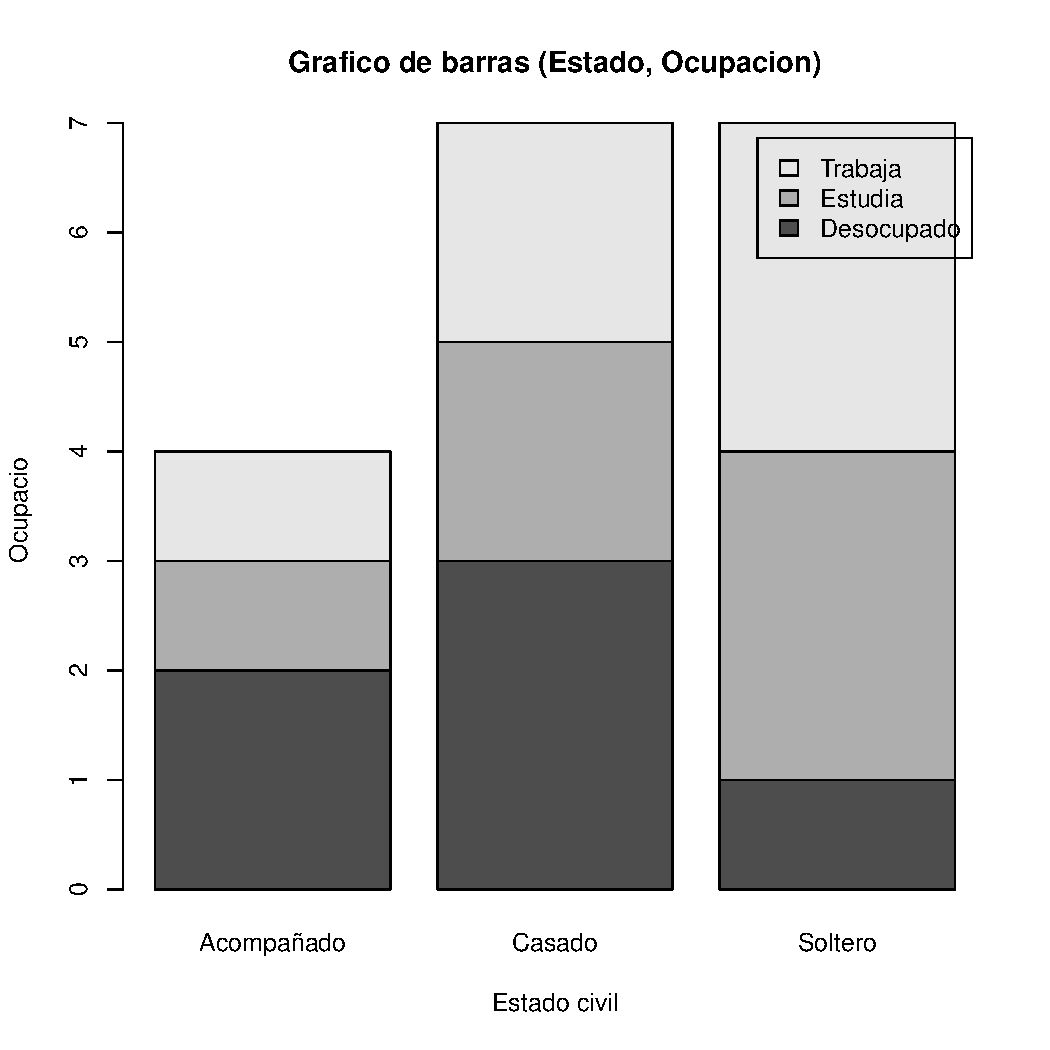
\includegraphics[width=\maxwidth]{figure/unnamed-chunk-1-1} 
\begin{kframe}\begin{alltt}
\hlstd{x} \hlkwb{<-} \hlnum{0}\hlopt{:}\hlnum{2}
\hlstd{m} \hlkwb{=} \hlnum{11}
\hlstd{n} \hlkwb{<-} \hlnum{4}\hlstd{; k}\hlkwb{=}\hlnum{2}
\hlcom{# x define el número de globos con premio}

\hlcom{# se construye la distribucion de frecuencias del numero de premios}
\hlstd{Tabla} \hlkwb{<-} \hlkwd{data.frame}\hlstd{(}\hlkwc{Probabilidad}\hlstd{=}\hlkwd{dhyper}\hlstd{(x, m, n, k))}
\hlkwd{rownames}\hlstd{(Tabla)} \hlkwb{<-} \hlkwd{c}\hlstd{(}\hlstr{"Ning�n premio"}\hlstd{,} \hlstr{"Solamente uno"}\hlstd{,} \hlstr{"Dos premios"}\hlstd{)}
\hlstd{Tabla}
\end{alltt}
\begin{verbatim}
##               Probabilidad
## Ning�n premio   0.05714286
## Solamente uno   0.41904762
## Dos premios     0.52380952
\end{verbatim}
\begin{alltt}
\hlstd{x} \hlkwb{=} \hlnum{1}\hlstd{; m}\hlkwb{=} \hlnum{10}\hlstd{; n}\hlkwb{=} \hlnum{3}\hlstd{; k}\hlkwb{=} \hlnum{2}\hlstd{;}
\hlkwd{dhyper}\hlstd{(x, m, n, k)}
\end{alltt}
\begin{verbatim}
## [1] 0.3846154
\end{verbatim}
\begin{alltt}
\hlcom{# x define el numero de intentos fallidos}
\hlstd{x} \hlkwb{<-} \hlnum{0}\hlopt{:}\hlnum{5}\hlstd{; p}\hlkwb{=}\hlnum{0.1}

\hlstd{Tabla} \hlkwb{<-} \hlkwd{data.frame}\hlstd{(}\hlkwc{Probabilidad}\hlstd{=}\hlkwd{dgeom}\hlstd{(x,} \hlkwc{prob}\hlstd{=p))}
\hlstd{Tabla}
\end{alltt}
\begin{verbatim}
##   Probabilidad
## 1     0.100000
## 2     0.090000
## 3     0.081000
## 4     0.072900
## 5     0.065610
## 6     0.059049
\end{verbatim}
\begin{alltt}
\hlcom{# nombrando las filas de la distribuci�n de frecuencias}
\hlkwd{rownames}\hlstd{(Tabla)} \hlkwb{<-} \hlkwd{c}\hlstd{(}\hlstr{"Venta en el primer intento"}\hlstd{,} \hlstr{"Venta en el segundo intento"}\hlstd{,}\hlstr{"Venta en el tercer intento"}\hlstd{,} \hlstr{"Venta en el cuarto intento"}\hlstd{,} \hlstr{"Venta en el quinto intento"}\hlstd{,} \hlstr{"Venta en el sexto intento"}\hlstd{)}
\hlstd{x}\hlkwb{=}\hlnum{0}\hlstd{; n}\hlkwb{=}\hlnum{7}\hlstd{; p}\hlkwb{=}\hlnum{0.1}
\hlkwd{dbinom}\hlstd{(x, n, p,} \hlkwc{log} \hlstd{=} \hlnum{FALSE}\hlstd{)}
\end{alltt}
\begin{verbatim}
## [1] 0.4782969
\end{verbatim}
\begin{alltt}
\hlstd{y} \hlkwb{<-} \hlnum{0}\hlopt{:}\hlnum{5}\hlstd{; r}\hlkwb{=}\hlnum{3}\hlstd{; p} \hlkwb{<-} \hlnum{0.1}
\hlstd{Tabla} \hlkwb{<-} \hlkwd{data.frame}\hlstd{(}\hlkwc{Probabilidad}\hlstd{=}\hlkwd{dnbinom}\hlstd{(y,} \hlkwc{size}\hlstd{=r,} \hlkwc{prob}\hlstd{=p))}
\hlkwd{rownames}\hlstd{(Tabla)} \hlkwb{<-} \hlnum{0}\hlopt{:}\hlnum{5}
\hlstd{Tabla}
\end{alltt}
\begin{verbatim}
##   Probabilidad
## 0   0.00100000
## 1   0.00270000
## 2   0.00486000
## 3   0.00729000
## 4   0.00984150
## 5   0.01240029
\end{verbatim}
\begin{alltt}
\hlcom{# Definir los par�metros apropiados}
\hlstd{n} \hlkwb{<-} \hlnum{15}\hlstd{; p} \hlkwb{<-} \hlnum{0.25}
\hlcom{# generar 100 n�meros aleatorios binomiales}
\hlstd{x} \hlkwb{=} \hlkwd{rbinom}\hlstd{(}\hlnum{100}\hlstd{, n, p); x}
\end{alltt}
\begin{verbatim}
##   [1] 3 4 3 5 6 2 5 4 2 3 2 4 5 3 3 7 4 2 2 4 1 3 3 4 2 6 3 2 5 2 5 4 3 4 3
##  [36] 3 7 2 3 4 2 4 7 3 8 1 4 4 5 4 6 4 5 3 5 2 4 5 4 3 2 3 1 2 2 4 6 1 2 7
##  [71] 2 1 2 3 3 6 5 2 0 8 2 5 5 3 4 6 2 5 4 4 6 0 4 1 6 5 3 1 1 4
\end{verbatim}
\begin{alltt}
\hlcom{# Histograma para la muestra aleatoria de tama�o 100}
\hlkwd{hist}\hlstd{(x,} \hlkwc{main}\hlstd{=}\hlstr{"X ~ Binomial(n=15, p=0.25)"}\hlstd{,} \hlkwc{xlab}\hlstd{=}\hlstr{"X = N�mero de �xitos"}\hlstd{,} \hlkwc{ylab}\hlstd{=}\hlstr{"masa de
probabilidad"}\hlstd{,} \hlkwc{probability}\hlstd{=}\hlnum{TRUE}\hlstd{,} \hlkwc{col}\hlstd{=}\hlstr{"blue"}\hlstd{)}
\hlstd{xvals}\hlkwb{=}\hlnum{0}\hlopt{:}\hlstd{n;} \hlkwd{points}\hlstd{(xvals,} \hlkwd{dbinom}\hlstd{(xvals, n, p),} \hlkwc{type}\hlstd{=}\hlstr{"h"}\hlstd{,} \hlkwc{lwd}\hlstd{=}\hlnum{3}\hlstd{)}
\hlkwd{points}\hlstd{(xvals,} \hlkwd{dbinom}\hlstd{(xvals, n, p),} \hlkwc{type}\hlstd{=}\hlstr{"p"}\hlstd{,} \hlkwc{lwd}\hlstd{=}\hlnum{3}\hlstd{)}
\end{alltt}
\end{kframe}
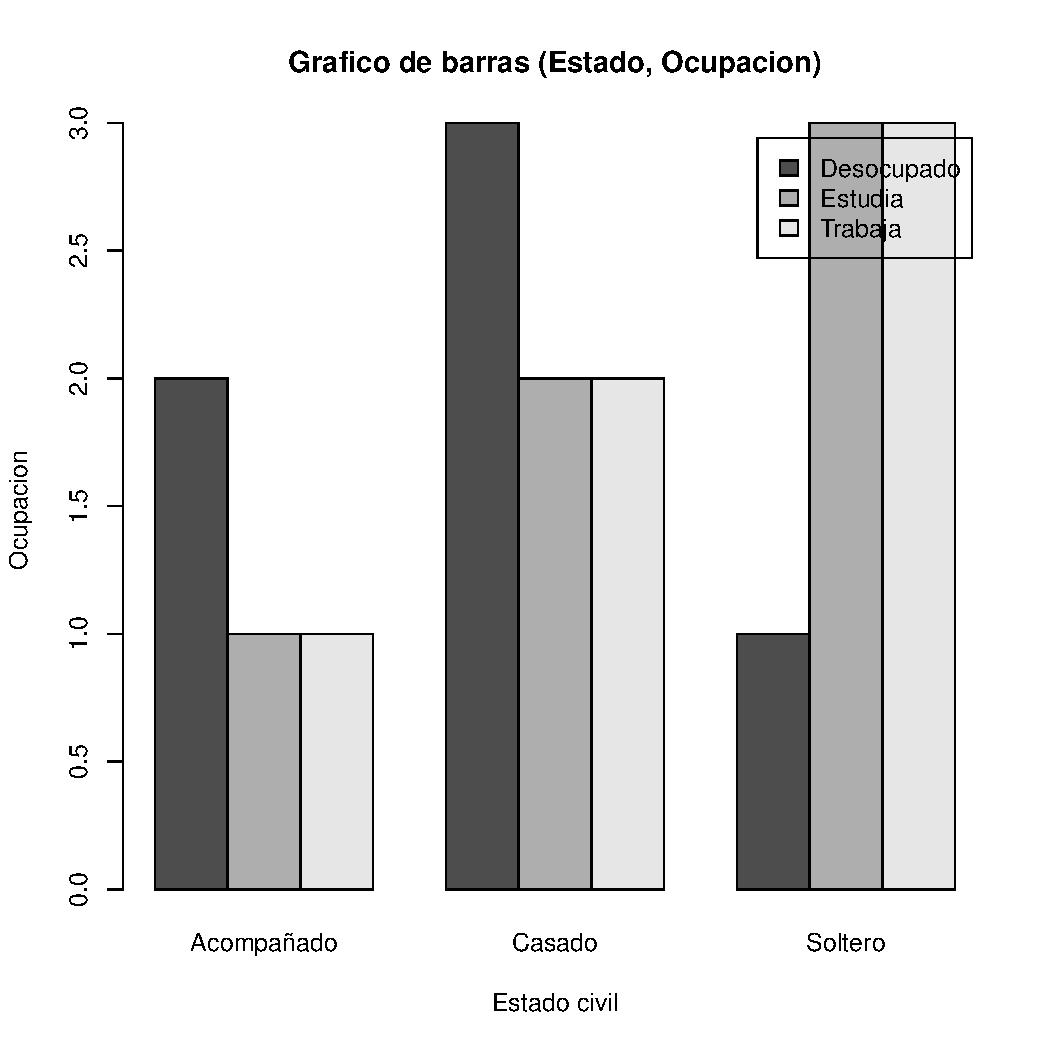
\includegraphics[width=\maxwidth]{figure/unnamed-chunk-1-2} 
\begin{kframe}\begin{alltt}
\hlcom{# Definir los par�metros apropiados}
\hlstd{n} \hlkwb{<-} \hlnum{200000}\hlstd{; p} \hlkwb{<-} \hlnum{3}\hlopt{/}\hlnum{100000}\hlstd{; lambda}\hlkwb{=}\hlstd{n}\hlopt{*}\hlstd{p}
\hlcom{# generar 100 n�meros aleatorios de la distribuci�n}
\hlstd{x} \hlkwb{=} \hlkwd{rpois}\hlstd{(}\hlnum{100}\hlstd{, lambda); x}
\end{alltt}
\begin{verbatim}
##   [1]  3  5  6  8  6  7  4  8  7  3  9  4  4  5  8  5  3  6  7  4 12  5  6
##  [24]  5  3  4  7  7  6  9  6  9  1 10 12  8  8  8  4  6  4  6  1  6  5  7
##  [47]  8  8  5  7  5  3  8  5  5  8  6  5  5  4  7  4  4  7  6  2  8  9  8
##  [70]  8  2  3 11  6  6  3  5  6  7  4  5  6  7 10  8  6  5  6  5  5  5  6
##  [93]  5 11  9  5 11  2  9  6
\end{verbatim}
\begin{alltt}
\hlcom{# Histograma para la muestra aleatoria de tama�o 100}
\hlkwd{hist}\hlstd{(x,} \hlkwc{main}\hlstd{=}\hlkwd{expression}\hlstd{(}\hlkwd{paste}\hlstd{(}\hlstr{"X ~ Poisson( "}\hlstd{, lambda,} \hlstr{" = 6 )"}\hlstd{)),} \hlkwc{xlab}\hlstd{=}\hlstr{"X = N�mero de eventos a
una tasa constante"}\hlstd{,} \hlkwc{ylab}\hlstd{=}\hlstr{"masa de probabilidad"}\hlstd{,} \hlkwc{probability}\hlstd{=}\hlnum{TRUE}\hlstd{,} \hlkwc{col}\hlstd{=}\hlstr{"blue"}\hlstd{)}
\hlstd{xvals}\hlkwb{=}\hlnum{0}\hlopt{:}\hlstd{n;} \hlkwd{points}\hlstd{(xvals,} \hlkwd{dpois}\hlstd{(xvals, lambda),} \hlkwc{type}\hlstd{=}\hlstr{"h"}\hlstd{,} \hlkwc{lwd}\hlstd{=}\hlnum{3}\hlstd{)}
\hlkwd{points}\hlstd{(xvals,} \hlkwd{dpois}\hlstd{(xvals, lambda),} \hlkwc{type}\hlstd{=}\hlstr{"p"}\hlstd{,} \hlkwc{lwd}\hlstd{=}\hlnum{3}\hlstd{)}
\end{alltt}
\end{kframe}
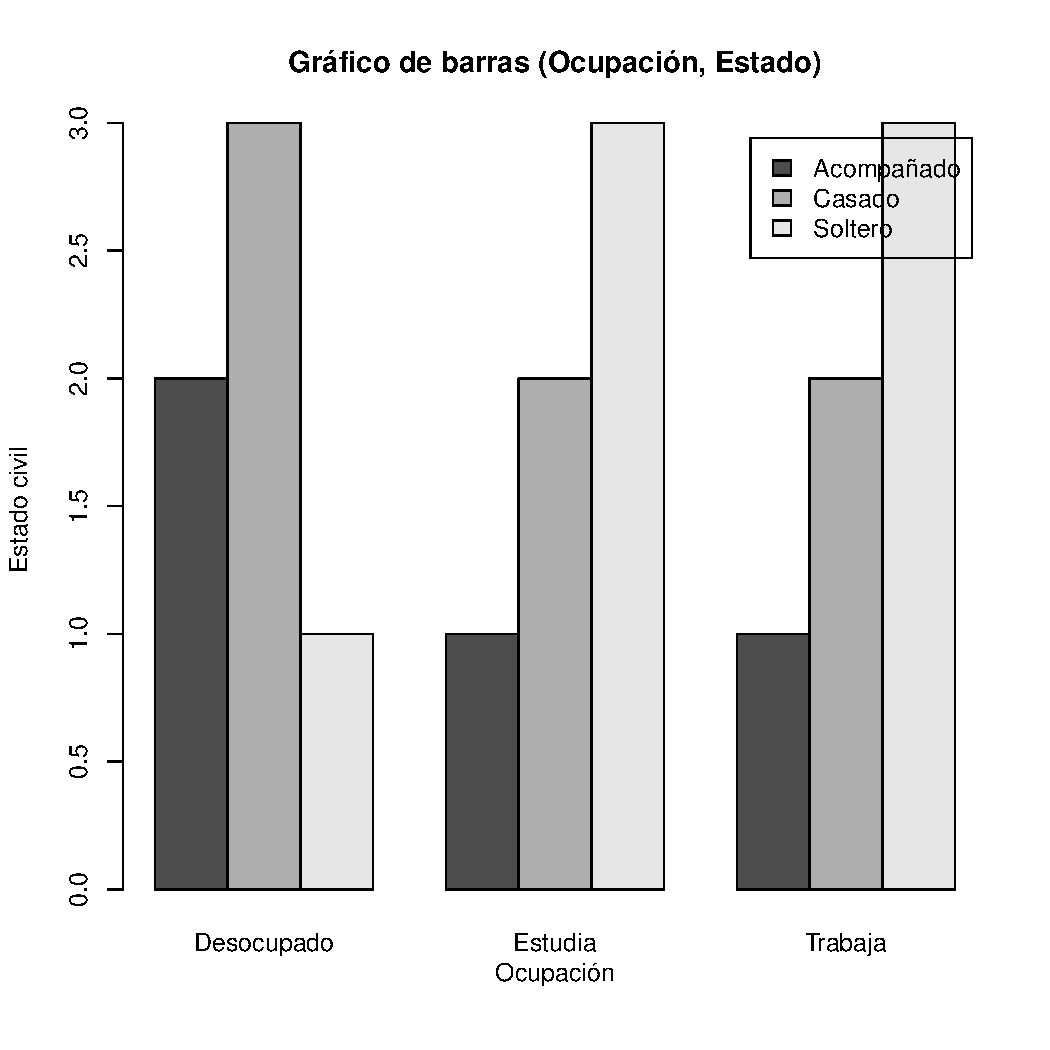
\includegraphics[width=\maxwidth]{figure/unnamed-chunk-1-3} 

\end{knitrout}



\end{document}
